% !TeX root = Thesis.tex

\chapter{Real~World~Use}
\label{chap:real_world_use}

We demonstrate an example of a real use case for CSG-CRN. Namely, we extract a point cloud from a video using photogrammetry and reconstruct a CSG model.

\section{Photogrammetry~Reconstruction}
\label{sec:photogrammetry_reconstruction}

A unique benefit of the point cloud input format for CSG-CRN is the flexibility in acquiring input data. Surface point clouds can be easily generated using photogrammetry techniques. And a surface point cloud can be augmented into an SDF point cloud input suitable for CSG-CRN.

To demonstrate, we took videos circling~360 degrees around three objects. An open-source tool, \texttt{COLMAP}~\cite{schoenberger2016sfm}, was used to extract frames, create depth maps, and output a point cloud scan. Some preprocessing is applied to the raw points to remove outliers, orient the shape into a canonical frame, and remove the floor plane. Similar to the ShapeNet dataset processing, near-surface sample points can be generated by applying Gaussian noise to the surface points. Distances for both near-surface and uniform points can be approximated using a K-d tree to find the closest surface sample.

We apply this process to produce three SDF shape samples to run inference on. We experiment with the single-category model trained on the ShapeNet car subset and the all-category model. The car subject is a known shape category that both models trained on while the rabbit and teddy bear subjects are unknown categories. Since there is no ground-truth mesh to validate against, we compute accuracy as the IoU metric between the reconstruction and input SDF point clouds.

The reconstructions and accuracy metrics are presented in Figure~\ref{fig:photogrammetry_renders}. As expected, the single-category model produced the best reconstruction of the four. It produced a smooth surface and a more defined windshield than the all-category model did. Both models were able to reconstruct the windows missing from the photogrammetry scan due to glare. The all-category model produced a decent approximation of the rabbit. The general shape is correct and contains a head and ears, but it lacks much detail. The reconstruction of the teddy bear sample is the worst result, with the model failing to reconstruct the arms and legs.


\begin{figure}[!htb]
	\centering
	\captionsetup[subfigure]{justification=centering}
	\begin{subfigure}{\textwidth}
		\centering
		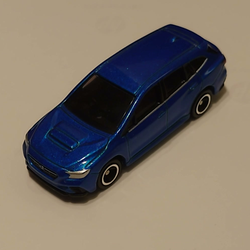
\includegraphics[width=0.13\textwidth]{Images/Photogrammetry Renders/Car Video Frame.png}
		\hspace{0.03\textwidth}
		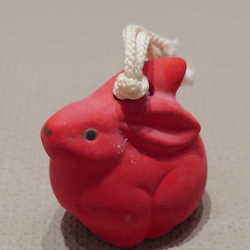
\includegraphics[width=0.13\textwidth]{Images/Photogrammetry Renders/Rabbit Bell Video Frame.png}
		\hspace{0.03\textwidth}
		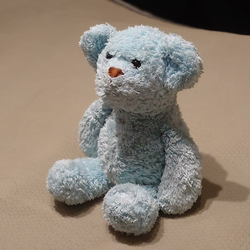
\includegraphics[width=0.13\textwidth]{Images/Photogrammetry Renders/Teddy Bear Video Frame.png}
		\caption{Video scan}
	\end{subfigure}
	
	\begin{subfigure}{\textwidth}
		\centering
		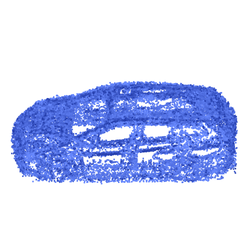
\includegraphics[width=0.13\textwidth]{Images/Photogrammetry Renders/Car Point Cloud.png}
		\hspace{0.03\textwidth}
		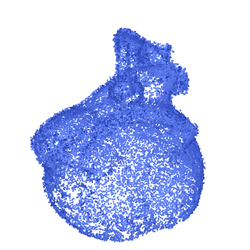
\includegraphics[width=0.13\textwidth]{Images/Photogrammetry Renders/Rabbit Bell Point Cloud.png}
		\hspace{0.03\textwidth}
		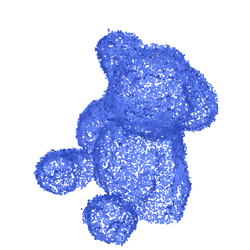
\includegraphics[width=0.13\textwidth]{Images/Photogrammetry Renders/Teddy Bear Point Cloud.png}
		\caption{Extracted point cloud}
	\end{subfigure}
	
	\begin{subfigure}{\textwidth}
		\centering
		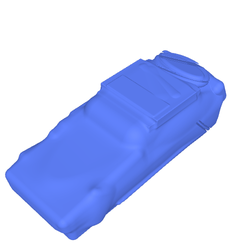
\includegraphics[width=0.13\textwidth]{Images/Photogrammetry Renders/Car Reconstruction Whole Dataset.png}
		\hspace{0.03\textwidth}
		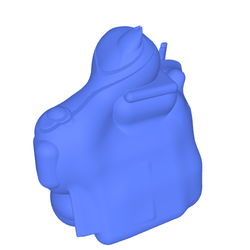
\includegraphics[width=0.13\textwidth]{Images/Photogrammetry Renders/Rabbit Bell Reconstruction.png}
		\hspace{0.03\textwidth}
		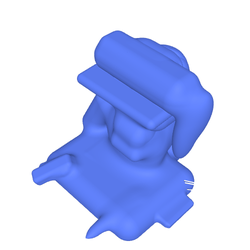
\includegraphics[width=0.13\textwidth]{Images/Photogrammetry Renders/Teddy Bear Reconstruction.png}
		
		\footnotesize
		\makebox[0.13\textwidth]{IoU 0.8865}
		\hspace{0.03\textwidth}
		\makebox[0.13\textwidth]{IoU 0.7252}
		\hspace{0.03\textwidth}
		\makebox[0.13\textwidth]{IoU 0.6242}
		\caption{All-category ShapeNet model reconstruction}
	\end{subfigure}
	
	\begin{subfigure}{\textwidth}
		\centering
		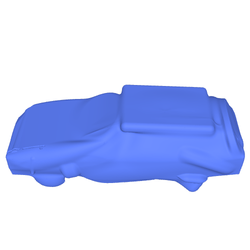
\includegraphics[width=0.13\textwidth]{Images/Photogrammetry Renders/Car Reconstruction Single Category.png}
		
		\footnotesize
		\makebox[0.13\textwidth]{IoU 0.8986}
		\caption{Single-category car model reconstruction}
	\end{subfigure}
	\caption{Reconstructing CSG models from video. The first row depicts frames from the video scan. The second row shows the surface point clouds extracted through photogrammetry. And the last two rows show CSG-CRN reconstructions.}
	\label{fig:photogrammetry_renders}
\end{figure}


\section{Test~Time~Optimization}
\label{sec:test_time_optimization}

The reconstruction results for the unseen shape categories rabbit and bear were significantly worse than for the seen shape category car. The accuracy for these shapes can be increased using Test Time Optimization (TTO)~\cite{Sun2020}. Before producing a reconstruction, the pre-trained model is further trained on the target shape. We create a dataset of one shape and optimize for~300 iterations before producing the reconstruction.

The improved results are presented in Figure~\ref{fig:photogrammetry_test_time_optimization}. The reconstructions are much cleaner for the rabbit and bear shapes which now have correct heads and ears. The car model did not improve much since the reconstruction without TTO was already highly accurate. The tradeoff for using this technique is that the time to reconstruct a shape grows from approximately~100~milliseconds to several minutes.

\begin{figure}[!htb]
	\centering
	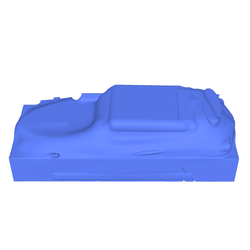
\includegraphics[width=0.13\textwidth]{Images/Photogrammetry Renders/Car Test Time Optimization.png}
	\hspace{0.03\textwidth}
	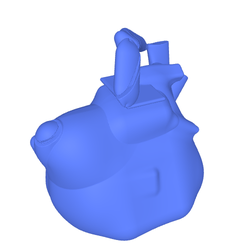
\includegraphics[width=0.13\textwidth]{Images/Photogrammetry Renders/Rabbit Bell Test Time Optimization.png}
	\hspace{0.03\textwidth}
	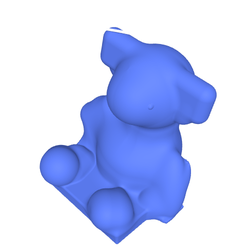
\includegraphics[width=0.13\textwidth]{Images/Photogrammetry Renders/Teddy Bear Test Time Optimization.png}
	
	{\footnotesize
		\makebox[0.13\textwidth]{IoU 0.9257}
		\hspace{0.03\textwidth}
		\makebox[0.13\textwidth]{IoU 0.8781}
		\hspace{0.03\textwidth}
		\makebox[0.13\textwidth]{IoU 0.8985}
		
	}
	\caption{All-category ShapeNet model with TTO reconstruction.}
	\label{fig:photogrammetry_test_time_optimization}
\end{figure}

\section{CSG~Export}
\label{sec:csg_export}

Lastly, the optimized reconstructions can be exported directly as a CSG model file without needing to remesh. The \texttt{MagicaCSG} CSG editor supports the roundness and blending parameters output by CSG-CRN. We provide an export utility to export a reconstruction in the .mcsg format so it can be imported and edited in \texttt{MagicaCSG}. A screenshot of the optimized bear reconstruction opened in \texttt{MagicaCSG} is shown in Figure~\ref{fig:magicacsg_teddy_bear}.

\begin{figure}[!htb]
	\centering
	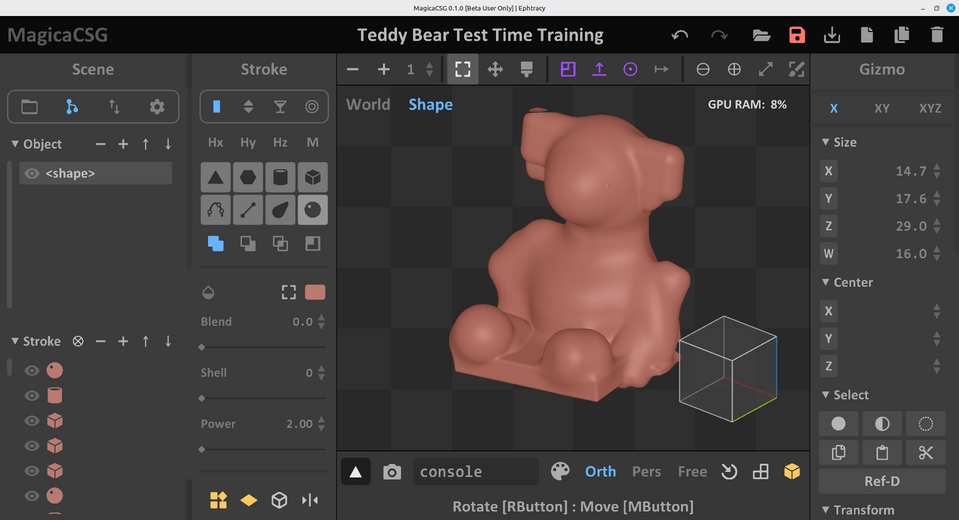
\includegraphics[width=\textwidth]{Images/Photogrammetry Renders/MagicaCSG Teddy Bear.png}
	\caption{Photogrammetry reconstruction imported into \texttt{MagicaCSG} as a CSG model.}
	\label{fig:magicacsg_teddy_bear}
\end{figure}
